%% abtex2-modelo-projeto-pesquisa.tex, v<VERSION> laurocesar
%% Copyright 2012-<COPYRIGHT_YEAR> by abnTeX2 group at http://www.abntex.net.br/ 

% ------------------------------------------------------------------------
% ------------------------------------------------------------------------
% abnTeX2: Modelo de Projeto de pesquisa em conformidade com 
% ABNT NBR 15287:2011 Informação e documentação - Projeto de pesquisa -
% Apresentação 
% ------------------------------------------------------------------------ 
% ------------------------------------------------------------------------

\documentclass[
	% -- opções da classe memoir --
	12pt,				% tamanho da fonte
	openany,			% capítulos começam em pág ímpar 	openright,			% capítulos começam em pág ímpar (insere página vazia caso preciso)
	oneside,			% para impressão em recto e verso. Oposto a oneside
	a4paper,			% tamanho do papel. 
	% -- opções da classe abntex2 --
	%chapter=TITLE,		% títulos de capítulos convertidos em letras maiúsculas
	%section=TITLE,		% títulos de seções convertidos em letras maiúsculas
	%subsection=TITLE,	% títulos de subseções convertidos em letras maiúsculas
	%subsubsection=TITLE,% títulos de subsubseções convertidos em letras maiúsculas
	% -- opções do pacote babel --
	english,			% idioma adicional para hifenização
	french,				% idioma adicional para hifenização
	spanish,			% idioma adicional para hifenização
	brazil,				% o último idioma é o principal do documento
	]{abntex2}

% ---
% PACOTES
% ---

% ---
% Pacotes fundamentais 
% ---
\usepackage{lmodern}			% Usa a fonte Latin Modern
\usepackage[T1]{fontenc}		% Selecao de codigos de fonte.
\usepackage[utf8]{inputenc}		% Codificacao do documento (conversão automática dos acentos)
\usepackage{indentfirst}		% Indenta o primeiro parágrafo de cada seção.
\usepackage{color}				% Controle das cores
\usepackage{graphicx}			% Inclusão de gráficos
\usepackage{microtype} 			% para melhorias de justificação
% ---

\usepackage{pdflscape} % provides the landscape environment

% ---
% Pacotes adicionais, usados apenas no âmbito do Modelo Canônico do abnteX2
% ---
\usepackage{lipsum}				% para geração de dummy text
% ---

% ---
% Pacotes de citações
% ---
\usepackage[brazilian,hyperpageref]{backref}	 % Paginas com as citações na bibl
\usepackage[alf]{abntex2cite}	% Citações padrão ABNT

% --- 
% CONFIGURAÇÕES DE PACOTES
% --- 

% ---
% Configurações do pacote backref
% Usado sem a opção hyperpageref de backref
\renewcommand{\backrefpagesname}{Citado na(s) página(s):~}
% Texto padrão antes do número das páginas
\renewcommand{\backref}{}
% Define os textos da citação
\renewcommand*{\backrefalt}[4]{
	\ifcase #1 %
		Nenhuma citação no texto.%
	\or
		Citado na página #2.%
	\else
		Citado #1 vezes nas páginas #2.%
	\fi}%
% ---

% ---
% Informações de dados para CAPA e FOLHA DE ROSTO
% ---
\titulo{ %
	Condições de Vida no Antropoceno:\\
	Cenários (capixabas) para um Brasil em 2030.}
\autor{Candidato Anônimo}
\local{São Paulo, Brasil}
\data{2016, v0.1}
\instituicao{ %
	\vspace{2cm}
	Universidade Federal do Espírito Santo - UFES \par
	Centro de Ciências Humanas e da Natureza - CCHN \par
	Programa de Pós-Graduação em Geografia \par 
	
%	\vspace{1.0cm}
%	\small{
%		\textbf{Natureza, Produção do Espaço e Território:}\par\vspace{-0.2cm}
%		\textbf{Estudos Urbanos e Regionais} \par\vspace{-0.2cm}
%		\textbf{Dinâmica dos Territórios e da Natureza} \par\vspace{-0.2cm}
%	}
	\vspace{2cm}
	\footnotesize{
		Prédio ``Profa. Bárbara Weinberg'' da Pós-Graduação \par \vspace{-0.2cm}
		CCHN Módulo I, sala 115 \par \vspace{-0.2cm}
		Av. Fernando Ferrari, 514, Goiabeiras \par \vspace{-0.2cm}
		Vitória, ES, 29.075-910 \par \vspace{-0.2cm}
	}
}
\tipotrabalho{Proposta para Projeto de Doutoramento}
% O preambulo deve conter o tipo do trabalho, o objetivo, 
% o nome da instituição e a área de concentração 
\preambulo{Projeto de pesquisa em conformidade
com as exigências do Programa de Pós Graduação e com as normas ABNT}
% ---

% ---
% Configurações de aparência do PDF final

% alterando o aspecto da cor azul
\definecolor{blue}{RGB}{41,5,195}
\definecolor{webbrown}{rgb}{0.65, 0.16, 0.16}
\definecolor{RoyalBlue}{rgb}{0.25, 0.41, 0.88}
\definecolor{forestgreen}{rgb}{0.13, 0.55, 0.13}


% informações do PDF
\makeatletter
\hypersetup{
     	%pagebackref=true,
		pdftitle={\@title}, 
		pdfauthor={\@author},
    	pdfsubject={\imprimirpreambulo},
	    pdfcreator={Marlon Pirchiner},
		pdfkeywords={abnt}{latex}{abntex}{abntex2}{projeto preliminar de pesquisa}, 
		colorlinks=true,       		% false: boxed links; true: colored links
		linkcolor=RoyalBlue, 
		citecolor=forestgreen,
%    	linkcolor=blue,          	% color of internal links
%    	citecolor=blue,        		% color of links to bibliography
    	filecolor=magenta,      		% color of file links
%		urlcolor=blue,
		urlcolor=webbrown,
		bookmarksdepth=4
}
\makeatother
% --- 

% --- 
% Espaçamentos entre linhas e parágrafos 
% --- 

% O tamanho do parágrafo é dado por:
\setlength{\parindent}{1.3cm}

% Controle do espaçamento entre um parágrafo e outro:
\setlength{\parskip}{0.2cm}  % tente também \onelineskip

% ---
% compila o indice
% ---
\makeindex
% ---

% ----
% Início do documento
% ----
\begin{document}

% Seleciona o idioma do documento (conforme pacotes do babel)
%\selectlanguage{english}
\selectlanguage{brazil}

% Retira espaço extra obsoleto entre as frases.
\frenchspacing 

% ----------------------------------------------------------
% ELEMENTOS PRÉ-TEXTUAIS
% ----------------------------------------------------------
% \pretextual

% ---
% Capa
% ---
\imprimircapa
% ---

% ---
% Folha de rosto
% ---
\imprimirfolhaderosto
% ---

% ---
% NOTA DA ABNT NBR 15287:2011, p. 4:
%  ``Se exigido pela entidade, apresentar os dados curriculares do autor em
%     folha ou página distinta após a folha de rosto.''
% ---

% ---
% inserir lista de ilustrações
% ---
%\pdfbookmark[0]{\listfigurename}{lof}
%\listoffigures*
%\cleardoublepage
% ---

% ---
% inserir lista de tabelas
% ---
%\pdfbookmark[0]{\listtablename}{lot}
%\listoftables*
%\cleardoublepage
% ---

% ---
% inserir lista de abreviaturas e siglas
% ---
%\begin{siglas}
%  \item[ABNT] Associação Brasileira de Normas Técnicas
%  \item[abnTeX] ABsurdas Normas para TeX
%\end{siglas}
% ---

% ---
% inserir lista de símbolos
% ---
%\begin{simbolos}
%  \item[$ \Gamma $] Letra grega Gama
%  \item[$ \Lambda $] Lambda
%  \item[$ \zeta $] Letra grega minúscula zeta
%  \item[$ \in $] Pertence
%\end{simbolos}
% ---

% ---
% inserir o sumario
% ---
%\pdfbookmark[0]{\contentsname}{toc}
%\tableofcontents*
%\cleardoublepage
% ---

\begin{resumoumacoluna}

Nessa proposta de pesquisa o conceito de Antropoceno é usado para situar o projeto em um contexto ambiental e natural mais amplo e unificador tanto das ciências naturais, por um lado, quanto das ciências humanas e sociais por outro. O que se convencionou por ciências do sistema terrestre, em que o Natural e o Humano são indissociáveis. Temas como governança e sustentabilidade parecem ter se tornado centrais. 
A revisão científica da agenda para 2030 das Nações Unidas, que marcam os objetivos globais para o desenvolvimento sustentável, serve de horizonte para seleção de modelos e perspectivas de análise.
O presente projeto preliminar de pesquisa apresenta propostas focadas na ciências da informação e organização do conhecimento como elemento aglutinador de saberes. 
Apresenta-se também uma perspectiva complexa de análise integrada da sociedade, território e espaço com objetivo de compreender e aprimorar as condições de vida. Com essa perspectiva espera-se poder simular dinâmicas sobre o uso do território em múltiplas escalas integrando saberes disponíveis para o apoio a processos decisórios e alocação de recursos.
Há, por isso, uma preocupação central com o local e regional, bem como em responder questões sobre desenvolvimento com horizonte sustável presentes nas agendas locais e regionais relacionados ao uso do território.
Observando-se até mesmo a própria dinâmica espacial desses conteúdos informativos. Uma meta espacialidade da informação. Uma preocupação com os lugares de produção, distribuição e difusão espacial da informação e dos saberes. %Interesses que se confundem muitas vezes com os do magistério superior.

 \vspace{\onelineskip}
 
 \noindent
 \textbf{Palavras-chave}: Território, Produção do Espaço, Natureza, Antropoceno, Ciências do Sistema Terrestre, Sistemas Complexos de Informação, Web Semântica, Ontologias, Dados Ligados, Engenharia do Conhecimento, Modelagem Computacional.
\end{resumoumacoluna}

% ----------------------------------------------------------
% ELEMENTOS TEXTUAIS
% ----------------------------------------------------------
\textual

% ----------------------------------------------------------
% Introdução
% ----------------------------------------------------------
\chapter[Introdução]{Introdução}
\addcontentsline{toc}{chapter}{Introdução}
%\begin{itemize}
%	\item breve apresentação do tema, com contextualização da proposta e trabalhos existentes na mesma temática; 
%	\item justificativas;
%	\item problemática (s).
%\end{itemize}


O Antropoceno \cite{crutzen_anthropocene_2000,crutzen_geology_2002}, embora ainda não formalmente aceito e incluído na Escala de Tempo Geológica \cite{gradstein_geologic_2005,cohen_ics_2013} (GTS, sigla em Inglês) da Comissão Internacional em Estratigrafia (ICS\footnote{International Comission on Stratigraphy \url{http://www.stratigraphy.org}.}, sigla também em inglês) é um conceito recente que, mesmo remontando de certa forma à teoria de \citeonline{lovelock_gaia_1979}, rompe o presente \cite{hamilton_anthropocene_2016} ao localizar a humanidade, coletivamente e de forma indelével \cite{zalasiewicz_new_2010,zalasiewicz_anthropocene:_2011} no Sistema Terra \cite{jacobson_earth_2000}. Mas ainda mais importante é que, embora algo sobre como quando exatamente teria sido seu início ainda esteja em aberto \cite{zalasiewicz_when_2015}, esse mote científico vem demonstrando que após meados do século XX teria ocorrido uma `grande aceleração' tanto em indicadores sócio-econômicos quanto naturais  \cite{steffen_anthropocene:_2011}. A essência unificadora desse conceito, em temas caros tanto às ciências Humanas quanto às Naturais, não só impulsiona o debate e a busca de uma solução conjunta como também evidencia, entre outras coisas, que com o atual ritmo do modo de produção global, com uma população crescente e diante da capacidade finita do ambiente, enquanto território em disputa política, de atender à crescente demanda por energia e outros recursos, não só influencia diretamente as condições de vida e desenvolvimento, como desafia a capacidade de governança para organizar um futuro menos desigual, mais inclusivo e sustentável.

Globalmente esse debate já vem sendo travado e, apesar das dificuldades inerentes ao processo, a apreciação pela comunidade científica e por entidades como o Conselho Internacional para a Ciência (ICSU\footnote{International Council for Science \url{http://www.icsu.org}.}, sigla em inglês) e o Conselho Internacional para Ciências Sociais (ISSC\footnote{International Social Science Council \url{http://www.worldsocialscience.org}.}, sigla também em inglês) de uma agenda com objetivos globais para 2030 em desenvolvimento sustentável vem sendo feita \cite{united_nations_transforming_2015,icsu-issc_review_2015}. A desigualdade, que contundentemente escancara nossas falhas de governança e alocação melhor distribuída de recursos, é apresentada como o primeiro dos objetivos: ``a eliminação de toda e qualquer forma de pobreza onde quer que houvesse''\cite{united_nations_transforming_2015}. 

Regional e localmente existem também muitos desafios de governança, com a produção do território, com uma melhor distribuição e alocação de investimentos. Recursos como por exemplo a água são fundamentais para a agricultura e para o abastecimento das cidades.

É nessa problemática, dos desafios de governança e políticas públicas para melhoria sustentável, e em múltiplas escalas, das condições sociais de vida agravadas pelo seu próprio modo de reprodução material, aparentemente contraditório à capacidade de suporte do ambiente, que essa proposta de pesquisa se insere. 

% ----------------------------------------------------------
% Capitulo de textual  
% ----------------------------------------------------------
\chapter{Objetivos}

\section{Objetivo Geral}

%O mais geral objetivo almejado pela pesquisa proposta é oferecer uma contribuição singela e singular sobre aspectos do ordenamento da Natureza e do ambiente 

O objetivo mais geral a ser atingido e proposto por essa pesquisa é apresentar cenários e estimativas de conformidade \cite{patterson_exploring_2016} com os objetivos globais para 2030 em desenvolvimento sustentável \cite{united_nations_transforming_2015} feitas à partir de uma perspectiva local.

Quando o problema central passa por temas como governança e proposição de políticas públicas, a produção, também pública, de conhecimento, informações e dados é mais do que necessária. É possível até mesmo defender a imprescindibilidade dessas atividades, sem as quais não é possível que haja uma justa avaliação das respostas às propostas e medidas adotadas.


\section{Objetivos Específicos}

A maioria, senão a totalidade, dos objetivos específicos dizem respeito, porém, ao modo pelo qual esses cenários e estimativas de conformidade pretendem ser desenvolvidos, entre eles:

\begin{enumerate}
	\item Investigar e avaliar o panorama atual de oferta de dados ambientais e sócio-econômicos ligados,
	\item Investigar e avaliar o uso de ontologias já desenvolvidas em contextos globais para modelar situações atuais de dados ambientais e socio-econômicos regionais e locais,
	\item Investigar e avaliar a aplicação de técnicas de Processamento da Linguagem Natural para extensão semântica de dados ligados com dados inicialmente não-estruturados,
	\item Investigar e avaliar modelos baseados em agentes para simulações de cenários de governança e desenvolvimento sustentável,
	\item Investigar e avaliar o uso integrado de tecnologias semânticas no consumo e assimilação contínua de dados em modelos de simulação social e otimização aplicados aos objetivos (ou pelo menos ao primeiro) locais e regionais para o desenvolvimento sutentável.
\end{enumerate}

% ----------------------------------------------------------
% Capitulo de textual  
% ----------------------------------------------------------
\chapter{Revisão Teórica}
\section{Discussão Bibliográfica (ou) Bases Conceituais}

Dados do Antropoceno evidenciam a presença inequívoca da influência humana no Sistema Terra e insustentabilidade dos modos atuais de produção além da conhecida limitação na capacidade de suprimento da demanda corrente, com a tecnologia disponível, e com as atuais projeções de crescimento. Não apenas podem não haver recursos necessários para as gerações futuras como sequer é garantido elevar-se a eficiência na distribuição e uso dos existentes, ao manter-se o ritmo atual.

Objetivos para o desenvolvimento, seja ele sustentável ou não, sempre foram objetos de agendas internacionais, nacionais, regionais e locais. Para 2030 as Nações Unidas apresentaram uma nova agenda com objetivos globais para o desenvolvimento sustentável. Destacado apenas o primeiro, a ``erradicação completa da pobreza sob todas as formas onde quer que houvesse''\cite{united_nations_transforming_2015} já é evidente os desfios de governança em múltiplas escalas.

Tendo sido enormemente ampliada a capacidade de observação da Terra, incluindo diversos elementos e aspectos da sociededade e de suas atividades, cresceu na mesma proporção a dificuldade em se recuperar informações confiáveis de diversas origens. As dificuldades de comunicação para fora do interior dos mais diversos domínios de conhecimento são evidentes. O símbolo $N$ seria apenas de força ou carregaria em sí certa qúimica? Lidar com dados e conceidos de múltiplas fontes requer cuidado extremo. A necessidade de informação é crescente, bem como a do profissional.

Além do aumento da importância nas disciplinas de informática \cite{fox_rise_2012} no contexto das pesquisas científicas tanto em ciências da Terra e do espaço como no campo das Humanidades, tecnologias semânticas vêm sendo amplamente discutidas por fóruns internacionais como a Aliança para Dados de Pesquisa (RDA\footnote{Research Data Alliance \url{https://rd-alliance.org}}, sigla em inglês) e o Consórcio Mundial da Rede (W3C\footnote{World Wide Web Consortium \url{https://www.w3.org/standards/semanticweb/}}, sigla também em inglês) vêm discutindo a apresentando boas práticas para usuários da comunidade científica.

A possibilidade de simular desdobramentos espaço-temporais do Sistema Terra, baseados em evidências, de decisões políticas e de governança em diversas escalas talvez tenha algo a contribuir nesse processo conjunto de desenvolvimento sustentável e redução das desigualdades com melhoria da condição de vida \cite{patterson_exploring_2016}. 

Estudos recentes do Instituto de Pesquisas Economicas e Aplicadas (IPEA) apontam na direção da complexidade social \cite{furtado_complexity_2015} e de maneiras para sua modelagem \cite{da_silva_territory_2015}. Já por outro lado, \citeonline{santos_o_2001} nos apresentam também uma visão intrigante acerca dos fluxos e da natureza do território e até mesmo para questões locais.

Finalmente, nos interessa em especial os recentes desenvolvimentos dos grupos de trabalho do Consórcio Global para a Internet (W3C\footnotetext{World Wide Web Consortium}, sigla em inglês) para dados espaciais \cite{w3c_spatial_2015} e suas boas práticas \cite{w3c_w3c_2015,taylor_where_2015}.


% ----------------------------------------------------------
% Capitulo de textual  
% ----------------------------------------------------------
\chapter{Materiais e Métodos}
\section{Materiais}

Há primazia por valer-se de dados produzidos por órgãos públicos que estejam abertos ou em processo de abertura.

Modelos integrados do sistema terrestre, com dados provenientes de múltiplos provedores e que façam uso intensivo de tecnologias semânticas exigem interoperabilidade por sua natureza. A forma amplamente reconhecida e mais recente de atingir os mais exigentes níveis de interoperabilidade tem sido através da anotação semântica com vocabulários e terminologias controladas, com a ligação (ou conexão) de conjuntos de dados às definições de seus conteúdos. É amplamente desejável, tornando-se quase necessário, que esses dados sejam confiáveis e também acessíveis por máquina.

Os provedores públicos de dados estruturados inicialmente cogitados serão enumeradas em seguida, sendo que os conjuntos específicos de dados devem ser definidos na medida em que forem sendo identificadas as informações mais relevantes para os modelos integrados. Inicialmente as próprias bases do Instituto Brasileiro de Geografia e Estatística (IBGE), seguidas por outras bases de interesse como IPEA (Instituto de Pesquisas Economicas Aplicadas), FGV (Fundação Getúlio Vargas), IBAMA (Instituto Brasileiro do Meio Ambiente), INPE (Instituto Nacional de Pesquisas Espaciais), ANA (Agência Nacional de Recursos Hídricos), ANTT (Agência Nacional de Transportes Terrestres), ANP (Agencia Nacional do Petróleo), CPRM (Serviço Geológico do Brasil), DNPM (Departamento Nacional de Produção Mineral), entre outros.

Incluir e disponibilizar publicamente o grafo de dados e informações utilizadas nos modelos diversificando as formas de consumo de dados e estatísticas públicas e também a visibilidade da escola e do instituto é um dos objetivos tácitos dessa pesquisa.

Ainda é preciso salientar os prováveis usos de informações não estuturadas, como corpus de publicações, textos jurídicos e legislações, além de documentos oficiais. Bases de dados como Scielo e Lattes são algumas das que estariam incialmente em vista.

\section{Métodos}

Investigar a existência de provedores e do estado dos dados públicos disponíveis nas perspectiva de \citeonline{berners-lee_linked_2006} e outros \cite{bizer_linked_2009} para dados ligados. A espectativa é de que seja possível reconhecer provedores de observações contínuas da natureza e do ambiente, do uso da terra, bem como dados sócio-econômicos em múltiplas escalas espaciais e temporais é uma das metodologias inicialmente consideradas para busca dos objetivos propostos. A identificação (e reúso), publicação e manutenção de vocábulários como forma de organização dos conhecimentos usando um sistema simples para organização do conhecimento (SKOS\footnote{Simple Knowledge Organization System \url{https://www.w3.org/TR/2009/REC-skos-reference-20090818/}}) deve facilitar a extração e publicação de conjuntos de dados com suas respectivas proveniências e metadados.

Além disso metodologias associadas ao campo das ciências da informação e documentação, bem como de engenharia e organização do conhecimento serão somadas para verificar as inserções e disponibilidade das tecnologias semânticas \cite{tim_berners-lee_james_hendler_and_ora_lassila_semantic_2001,berners-lee_publishing_2001,narock_science_2012,ma_semantic_2015,mattoso_addressing_2016} e das ciência da informação \cite{baker_egy:_2009, fox_rise_2012} em ampliar as capacidades de interoperabilidade \cite{cardoso_semantic_2003} sem contudo perder em confiabilidade \cite{gil_towards_2007} e reprodutibilidade \cite{mattoso_addressing_2016} com o uso conveniente da proveniência \cite{lebo_prov-o:_2013} em conjuntos de dados.

Metodologias complementares seriam adotadas para atingir objetivos, por exemplo, acerca da disponibilidade de ontologias, ou representações formais do estado e da evolução do conhecimento, da terminologia, dos conceitos, relacionamentos, podendo também expressar restrições lógicas, nos domínios científicos de conhecimento específico que versem ou se relacionem com dados e modelos de desenvolvimento existentes. O que seria uma abordagem dedutiva para a representação do saber-fazer científico, codificação rigorosa de metodologias e divulgação de resultados \cite{patton_semnext:_2015,mattoso_addressing_2016,diviacco_collaborative_2015}.

Para idealizar e desenvolver um fluxo de trabalho, utilizando-se do Processamento da Linguagem Natural para dar estrutura a conjuntos de dados não estruturados já existem muitos mecanismos e literatura desenvolvida. Basicamente pretende-se seguir a linha desenvolvida pelo grupo da Universiade de Stanford\footnote{Stanford NLP Group \url{http://nlp.stanford.edu}}. Técnicas como modelagem probabilística de tópicos \cite{blei_probabilistic_2012} tendem a ser bastante relevantes assim como de alinhamento baseado em similaridades. Um exemplo de aplicação seria para anotação e busca semântica de documentos. Esse fluxo se pretende complementar e aumentar o grafo de conhecimento numa abordagem abdutiva que impulsiona mais descobertas e inovações \cite{gil_data_2009}.

Teorias, metodologias e publicações na linha de \citeonline{jones_design_2013} e \citeonline{pitt_interleaving_2011} tendem incialmente ocupar um bom espaço e tempo de reflexão. Ao se investigar e avaliar o estado da arte de modelos baseados em agentes para simular reações e desdobramentos de cenários futuros \cite{da_silva_territory_2015}, talvez seja necessário também desenvolver e acrescentar condicionantes ambientais à axiomatizações como as de \citeonline{pitt_axiomatization_2012}.

Sendo um dos objetivos mais audaciosos dessa proposta, muito ainda deve ser acrescido ao que foi considerado até o momento para se investigar e avaliar o uso conjunto de fluxos semânticos de trabalho \cite{mattoso_addressing_2016} modelos baseados em agentes no suporte à decisões sobre questões de governança e sustentabilidade \cite{buckingham_shum_towards_2012}, principalmente no que se refere à necessidade de interligar o universo descritivo e numérico dos problemas \cite{patton_semnext:_2015}.

% ----------------------------------------------------------
% Capitulo de textual  
% ----------------------------------------------------------
\chapter{Metas e Cronograma de Atividade}
\section{Metas}

Entre os resultados esperados mais elementares dessa pesquisa encontram-se um panorama sobre o estado de desenvolvimento das tecnologias semânticas e de dados ligados para interoperabilidade disponíveis no Brasil e no Espírito Santo.

Espera-se também poder contribuir com o desenvolvimento e expansão de um grafo público de conhecimento relacionado à população, território e condições de vida no Brasil e no Espírito Santo.

A avaliação sobre em que extensão as tecnologias semânticas poderiam contribuir tanto para a melhoria da comunicação e ampliação do entendimento no diálogo entre discliplinas dos campos Humano e Natural.

A pesquisa prentende resultar também em uma avaliação crítica das possibilidades do aumento da riqueza e da quantidade de informações através do processamento (por máquina) da linguagem natural por dar certa estrutura e sentido semântico à quantidades antes inacessíveis de informação.

Espera-se, ao longo dos anos de execução, dar maior atenção aos modelos baseados em agentes para simulações e inferências sobre cenários futuros a partir da observação e amostragem de diversas séries de dados espaço-temporais.

Por fim, espera-se contribuir, com precisão e confiabilidade das informações apresentadas e/ou recomendadas em diferentes escalas, para o avanço em direção à conquista dos objetivos globais para o desenvolvimento sustentável, no marco de 2030, mas que exigem, desde há muito, organização e ações coletivas em escalas regionais e locais.

\newpage
\section{Cronograma de Atividades}

A tabela \ref{tab:workingplan} abaixo, apresenta o cronograma inicialmente proposto para as atividades agrupadas segundo a natureza das atividades. Na presente versão da proposta, este cronograma, dividido em oito semestres, apresenta tão somente uma tentativa para a organização da execução das atividades futuras.

%\begin{landscape}
%	\thispagestyle{empty}
%	\centering
	\begin{table}[h]
		%\hspace{-1.5cm}
		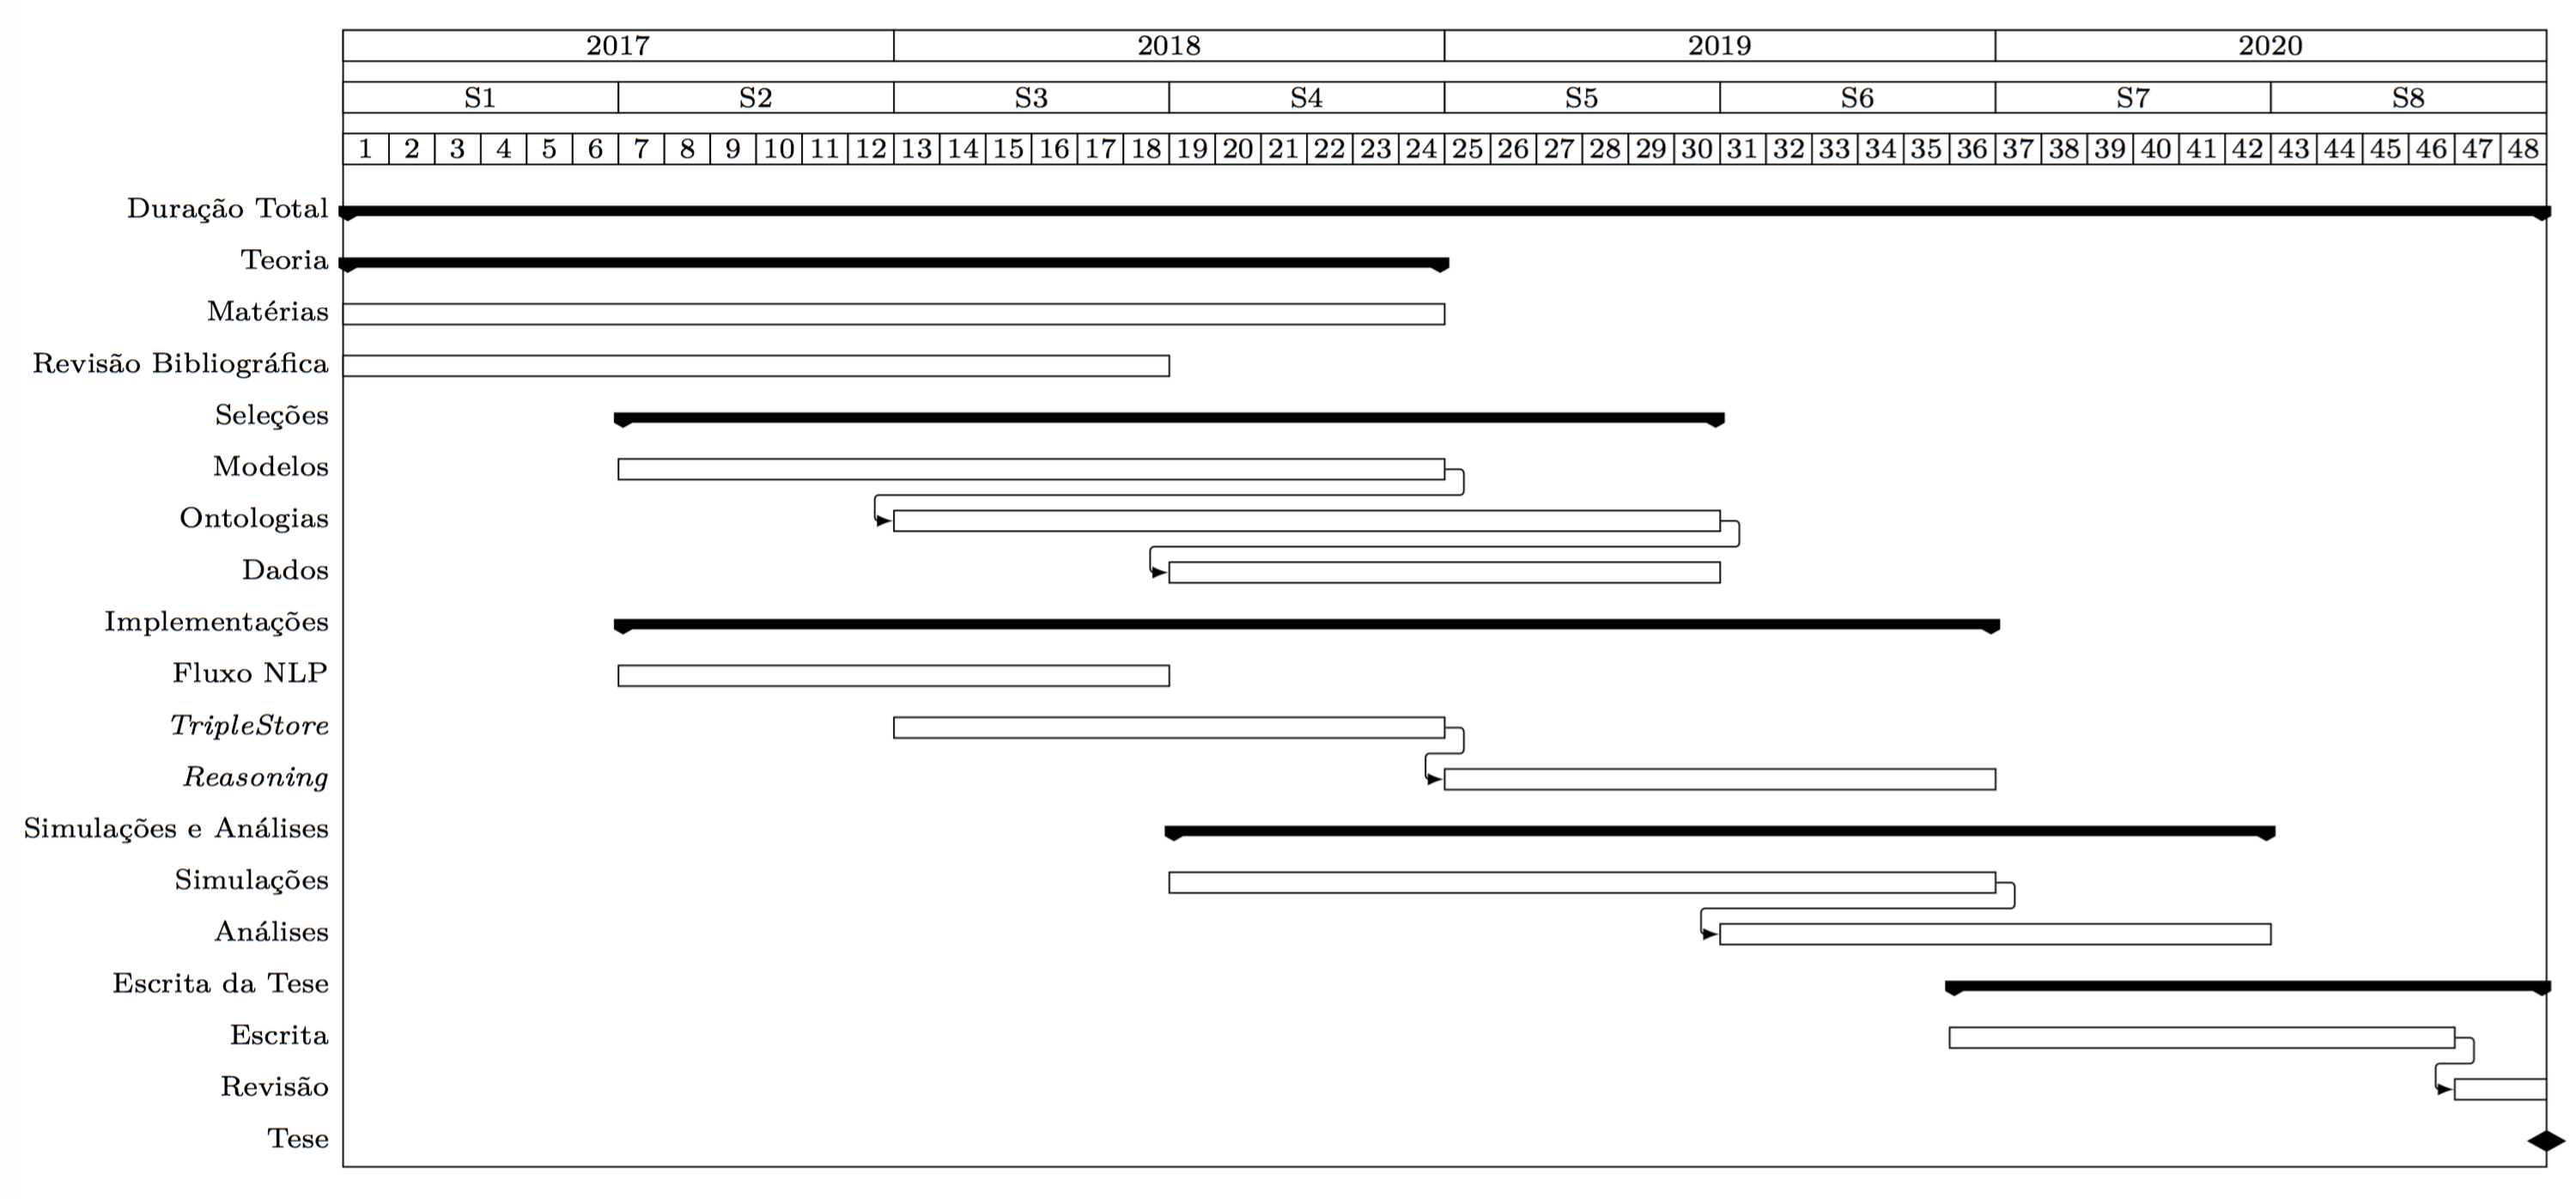
\includegraphics[width=1.00\columnwidth]{timetable_png} 
		\caption[Cronograma de Atividades]{Cronograma de Atividades} 
		% The text in the square bracket is the caption for the list of figures while the text in the curly brackets is the figure caption
		\label{tab:workingplan} 
	\end{table}
%\end{landscape}
No cronograma da tabela \ref{tab:workingplan} é possível identificar uma primeira fase teórica que inclui também as disciplinas do curso. Há uma fase para seleção dos modelos que serão simulados e das ontologias que serão utilizadas para mapear os dados ligados. Uma fase de implementação, tanto do fluxo de Processamento da Linguagem Natural (NLP, sigla em inglês), quanto do banco de ``triplas'' (do original \emph{triple store} em inglês) contendo o grafo de conhecimento e além do ``raciocínio'' semântico. Uma fase em separado para as análises e simulações. O último grupo de atividades correspondem a síntese e escrita da tese propriamente com um tempo reservado ao final para as revisões.




\chapter{Viabilidade e Disponibilidade}

\section{Viabilidade}
Inicialmente o projeto poderia ser prototipado em um computador pessoal com acesso à Internet e recurso para \emph{back-up}. Posteriormente seria possível aumentar a escala de processamento conforme a necessidade.

A viabilidade executiva do projeto pode ser verificada pela existência de dados, ontologias e modelos. 

A viabilidade financeira do projeto poderia ser estimada com detalhes em dependência da pré-existência de recursos computacionais e da capacidade de se estabelecer relações futuras que possam auxiliar na solução de algum eventual aumento de demanda. 

\section{Disponibilidade}

A disponibilidade do candidato para o desenvolvimento mais ou menos eficiente do projeto ficaria condicionada à bolsa de pesquisa.


% ---
% Finaliza a parte no bookmark do PDF
% para que se inicie o bookmark na raiz
% e adiciona espaço de parte no Sumário
% ---
\phantompart

% ---
% Conclusão
% ---
\chapter*[Considerações finais]{Considerações finais}

A presente proposta é ainda um documento em construção. Foi iniciado, no contexto de reunir, ainda de forma bem aberta mas também com certo grau de detalhamento técnico, informações que abrissem um diálogo sobre os interesses, capacidade de articulação e possibilidades a serem exploradas conjuntamente no futuro caso haja interesse recíproco e sendo, é claro, o candidato selecionado e aprovado pelo processo seletivo neste ano de 2016 para o ano de 2017. Não se trata portanto de um documento elaborado após uma exaustiva pesquisa ou um aprofundado detalhamento do que venha a ser de fato desenvolvido. 

Parece importante que haja espaço para contribuições diversas, sejam do próprio candidato, com um trabalho mais pormenorizado, sejam as de professores colaboradores que tenham interesse e venham eventualmente se envolver um pouco mais ou até mesmo dos que com ou sem experência acabem, voluntariamente ou não, deixando sua contribuição.

Espero que mesmo simplificadamente uma mensagem minimamente clara de interesse pelo objeto Humano e Social na pesquisa e em suas relações com o Natural e o Espacial, principalmente quando desenvolvida a partir de métodos formais e tecnologicamente desafiadores.

% ----------------------------------------------------------
% ELEMENTOS PÓS-TEXTUAIS
% ----------------------------------------------------------
\postextual

% ----------------------------------------------------------
% Referências bibliográficas
% ----------------------------------------------------------
\bibliography{phd}


\end{document}
